\documentclass[sigconf]{acmart}
\usepackage{cleveref}
\usepackage{graphics}
\settopmatter{printacmref=false}
\setcopyright{none}
\renewcommand\footnotetextcopyrightpermission[1]{}
\pagestyle{plain}
\crefformat{section}{\S#2#1#3}

\definecolor{codegreen}{rgb}{0,0.6,0}
\definecolor{codegray}{rgb}{0.5,0.5,0.5}
\definecolor{codepurple}{rgb}{0.58,0,0.82}
\definecolor{backcolour}{rgb}{0.95,0.95,0.92}

\def\authnote{1}


\usepackage{listings}
\usepackage{xcolor}
\usepackage{upquote}

%New colors defined below
\definecolor{codegreen}{rgb}{0,0.6,0}
\definecolor{codegray}{rgb}{0.5,0.5,0.5}
\definecolor{codepurple}{rgb}{0.58,0,0.82}
\definecolor{backcolour}{rgb}{0.95,0.95,0.92}

%Code listing style named "mystyle"
\lstdefinestyle{mystyle}{
  backgroundcolor=\color{backcolour},   commentstyle=\color{codegreen},
  keywordstyle=\color{magenta},
  numberstyle=\tiny\color{codegray},
  stringstyle=\color{codepurple},
  basicstyle=\ttfamily\footnotesize,
  breakatwhitespace=false,         
  breaklines=true,                 
  captionpos=b,                    
  keepspaces=true,                 
  numbers=left,                    
  numbersep=5pt,                  
  showspaces=false,                
  showstringspaces=false,
  showtabs=false,                  
  tabsize=2,
  keepspaces=true,
  language=java
}

\lstset{style=mystyle}


\usepackage[most]{tcolorbox}

%textmarker style from colorbox doc
\tcbset{textmarker/.style={%
        enhanced,
        parbox=false,boxrule=0mm,boxsep=0mm,arc=0mm,
        outer arc=0mm,left=6mm,right=3mm,top=7pt,bottom=7pt,
        toptitle=1mm,bottomtitle=1mm,oversize}}


% define new colorboxes
\newtcolorbox{hintBox}{textmarker,
    borderline west={6pt}{0pt}{yellow},
    colback=yellow!10!white}
\newtcolorbox{importantBox}{textmarker,
    borderline west={6pt}{0pt}{red},
    colback=red!10!white}
\newtcolorbox{noteBox}{textmarker,
    borderline west={6pt}{0pt}{green},
    colback=green!10!white}

% define commands for easy access
\newcommand{\note}[1]{\begin{noteBox} \textbf{Note:} #1 \end{noteBox}}
\newcommand{\warning}[1]{\begin{hintBox} \textbf{Warning:} #1 \end{hintBox}}
\newcommand{\important}[1]{\begin{importantBox} \textbf{Important:} #1 \end{importantBox}}




\newcounter{mynote}[section]
\newcommand{\notecolor}{blue}
\newcommand{\thenote}{\thesection.\arabic{mynote}}
\newcommand{\tnote}[1]{\ifnum\authnote=1\refstepcounter{mynote}{\bf \textcolor{\notecolor}{$\ll$TomR~\thenote: {\sf #1}$\gg$}}\fi}

\newcommand{\fixme}[1]{\ifnum\authnote=1{\textcolor{red}{[FIXME: #1]}}\fi}
\newcommand{\better}[1]{\ifnum\authnote=1{\textcolor{violet}{[BetterWord: #1]}}\fi}
\newcommand{\todo}[1]{\ifnum\authnote=1{\textcolor{red}{[TODO: #1]}}\fi}

\newcommand{\new}[1]{\textcolor{blue}{#1}}

%% ------------------------- Damon -----------------------

\newcommand{\minote}[1]{{\bf \textcolor{red}{$\ll$Mazharul~\thenote: {\sf #1}$\gg$}}}



\begin{document}
%%
%% The "title" command has an optional parameter,
%% allowing the author to define a "short title" to be used in page headers.
\title{Suggesting Secure Implementation to Vulnerable Code Snippets on Stackoverflow.}
\begin{abstract}
\begin{abstract}
Online programming discussion platforms such as Stack Overflow have a rich source of ready to use code snippets for software developers. 
It is the de fac-to place where developers go to find solutions. %from the coding snippets given as answers to posted problems by the online developer community. 
However, previous research work has shown that developers have a tendency to directly copy-paste insecure code snippets from 
Stack Overflow into their production level code. 
As a result without any countermeasures Stack Overflow is becoming one of major sources of causing vulnerabilities in production level source code. 
To address this problem, in this project, we tackle the problem of analyzing code snippets found on Stack overflow. 
This is challenging since code snippets from Stack overflow are often-times erroneous, incomplete, and lack dependencies which makes 
it harder to analyze them by state-of-the-art static tools.
In this paper we identify 8 common insecure patterns by analyzing a collection of 1.6K code snippets from Stack Overflow. 
We use a combination of keyword searching and backward flow analysis to detect these 8 common insecure patterns. 
We believe that by identifying the common insecure patterns in code snippets, found online programming discussion platforms websites such as Stack Overflow,  
it is possible to encourage developers to write secure code snippets, and discourage them from copy-pasting insecure code snippets
into production level source code.
\end{abstract}  
\end{abstract}
\maketitle
\section{Introduction}
%\tnote{This is a message.}
   \label{into}
   %\minote{Add a ss from stackOverflow}

   \begin{figure}
   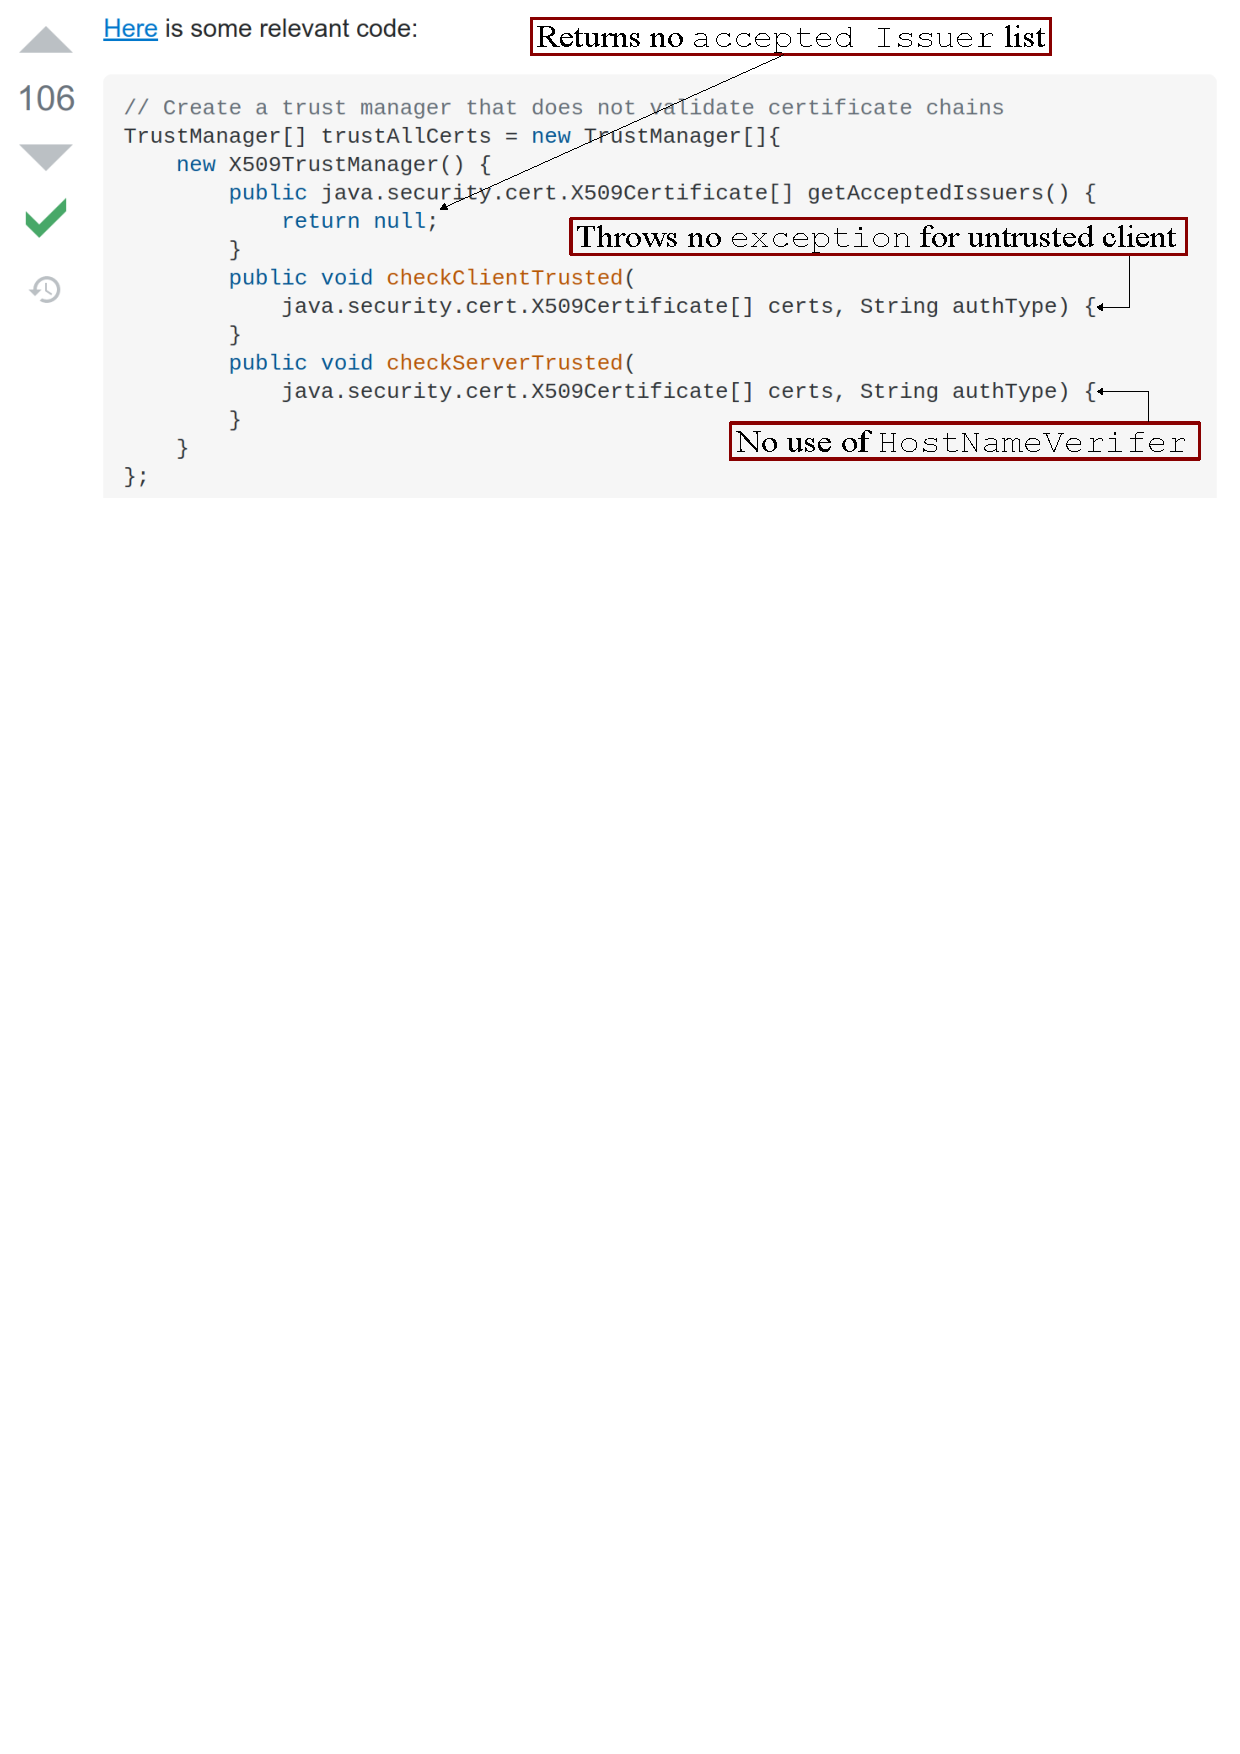
\includegraphics[width=\linewidth]{Figures/SO_ss.png}
   \caption{}
   \label{fig:SO_screenshot}
   \end{figure}
   
   %\textcolor{blue}{we can't also using testing to test the code snippet mention it somewhere...}
   %\note{Certainly elsewhere my do allowance at. The address farther six hearted hundred towards husband. Strangers ye to he sometimes propriety in. She right plate seven has. Bed who perceive judgment did marianne.}
   Stack Overflow (SO) is regarded as one of the most popular online helping platforms for software developers~\cite{8816778}. 
   SO seeks to help by creating an eco-system of online developer community. 
   In this ecosystem one developer can ask for solutions to the to the problems one is facing, while other developers can interact by posting code snippets, advices, as solutions to those asked problems. 
   As such SO has become a rich source of ready to use code snippets for software developers. 
   This richness has caused SO to enter the agile software development cycle allowing prototyping, and an efficient workflow. Particularlly inexperienced programmers treasure the direct help from the community providing easy ready-to-use code snippets.
   Interesting copying code snippets into production software is generally practiced not only by the novice but a common practice shared by large parts of the developer community. Furthermore, sometimes experienced developers can potentially promote distribute best- practices and may improve code quality on a large basis.
   %Because whenever developers search online to find a working solution %to the problem they are facing, 
   %they are very likely to encouter an accepted working code snippet in SO to solve that problem. 
   %post created by some developer who has faced the same problem previously.

   Unfortunately this is not same for secure coding practices. Fischer et al.~\cite{fischer2017stack} quantitatively evaluated that an Android developer seeking help can find accepted popular code snippets suggesting insecure X.509 certificate validation, misusing Android’s cryptographic API (Figure~\ref{fig:SO_screenshot}). Moreover a developer struggling with handling Java Spring security framework's configuration errors can find code snippets suugessting turning off CSRF security protection entirely to avoid errors. Insecure code snippets found on Stackoverflow itself is not a serious problem. However insecure code snippets are being upvoted, accepted by the online developer community, even so by users with high repuration~\cite{meng2018secure}. Therefore these insecure code snippets are naturally entering the development cycle by developers copy-pasting them into the production level code -- casuing vulnerabilities in softwares.

   
   
   However there is no existing tool used by SO to analyzie and flag a code snippet if it contains potential insecure secure patterns.
   This type of flagging can make the developers more aware before upvoting the code snippets or copy pasting into their own production level code base. Moreover this will also encourage, and cause the high repulated users to pay special attention to write secure code snippets as answers. 
   
   Towards this goal in this paper we aim to develop a static analysis tool  which can identify which part of the code snippet is insecure and suggest secure alternative suggestions to write it securely. However analyzing code snippets for insecure patterns presents some unique challenges. Since  code snippets are erronous, incomplete, we have apply repair techniques to convert them to an intermidate representation (IR). 
   To address this problem, we first studied the literature to compile a list of 8 most insecure patterns related to code snippets in Java languagewe. We then applied simple parsing repairs to the code snippets, and used a combination of keyword and backword flow analysis based detection method. 
   
   In summary, the contributions of the paper are the following: 
   \begin{itemize}
   \item We survey the literature, and present 8 most insecure patterns appering recursively in Java language code snippets posted on SO. (section ~\ref{sec:insecure-patterns})      
   \item We repaired the code snippets from SO, and convert them to Jimple intermidate representation (IR) to detect the 8 insecure patterns. (section~\ref{subsec:code-repair}) 
   \item  We developed keyword and backword flow analysis based detection method to identify the presence of 8 insecure patterns.
   \item Results
   \end{itemize}
   %Then we can run analysis on the IR. In this paper we apply simple parsing repairs to 1.6K , used  
   %In absense of such tool, SO is potentially contributing as a major source of vulnerability in production level code.        

   % TODO: Integrating into SO?
   %\iffalse
   %\begin{itemize}
   %\item  Analyze the code snippets from Stackoverflow for identifying out which part of the code is vulnerable by showing warning signs to highlight that part of the code to the developer.
   %\item When developer clicks on the warning sign a secure implementation while be shown to the developers. In case of failure of building generating a secure implementation, the tool will show insightful/helpful messages explaing why this part of the code is flaged as insecure.  
  % \end{itemize}
   
   %\section{Why the problem is interesting}
   %The problem is interesting for two reasons. 
   
   %\paragraph{Difficulty of writing crypto code securely.} Writing/implementing cypto code securely is a diffculut task for programmers. Any potential bug in crypto code can lead to serious vulnerablities open for attackers.
   %Even so unlike other code, crypto code can be insecure even if it works 
   %perfectly on traditional test-suite's input/output which is used only to prove the implementation correctness of the program.
   
   %\paragraph{Online platforms roles in spreading insecure code.} Online programming discussion platforms such as Stack Overflow have a rich source of ready to use code snippets for software developers. It is the defac-to place where developers go to find solutions of their problems and turn to the community for answers to their problems. 
   %Insecure code snippets found on Stackoverflow itself is not a serious problem. However,  
   %Fischer et al. has shown that developers have a tendency to directly copy paste code form Stack Overflow~\cite{fischer2017stack}. 
   %Therefore there are chances that any insecure code snippets posted on Stackoverflow can potentially find it way into production level code. To make matters worse, Meng et al.~\cite{meng2018secure} has showed that many accepted answers on Stackoverflow have seriously insecure code and often-times given by users having high reputation. This adds to the problem copy pasting vulnerable code from online platform and furthermore increases the chances of the insecure code snippet being trickled down to production level code. 
   %Unfortunately there is not state-of-the-art tool to analyzie if a code posted by developer on Stackoverflow is secure or not. 
   %In absense of such tool, Stackoverflow is potentially contributing as a major source of vulnerability in production level code.  
   
   %A static tool which can identify which part of the code snippet is insecure and suggest secure alternatives can help stopping 
   %the flow of insecure code from Stackoverflow to production level code.

   %\minote{Talk about key challenges here. Say there are existing tools that can detect these rules on complete source codes.  
   %But code snippets presents some unique challenges. such has
   %\begin{itemize}
   %   \item code snippets are erronous
   %   \item code snippets are incomplete  
   %\end{itemize}
   %}
   %\fi   
\section{Threat model}
\section{Threat Model}
\label{sec:insecure-patterns}
%Kye insights
%\begin{itemize}
%  \item Limit analysis to some specifice crypto functions.
%  \item For rule 1, 2, 7, 8 we just did a keyword search on methods we are interested in.
%  \item For 4, 5, 6, 7 we have to do a backward flow analysis. 
%\end{itemize}

\begin{table}[ht]
 %\resizebox{\linewidth}{!}{
   \scriptsize
\begin{tabular}{|l|l|l|l|}
  \toprule
  \begin{tabular}[c]{@{}l@{}}Insecure\\Pattern \#\end{tabular} & Description                                  & Vulnerability  \\ \midrule 
  1                                                 & AES default encryption mode ECB              & Side channel attack    \\ 
  2                                                 & Insecure cryptographic hash                  & Collision attack    \\  
  3                                                 & Abuse of X509TrustManager Verifier Interface & \multicolumn{1}{c|}{SSL/TLS MitM attack} \\ 
  4                                                 & Weak key length                              & Brute force attack   \\ 
  5                                                 & Static/constant/predictable keys/IV          &                   \\ \midrule
  7                                                 & Presence of AllHostNameVerifier              & SSL/TLS MiTM \\                                         
  8                                                 & Turning of CSRF protection                   & CSRF attack \\
  \bottomrule
  \end{tabular}
  \caption{The 8 most insecure patterns found on code snippets from Stack Overflow}
  \label{tab:insecure-patterns}
% }
\end{table}
%%%Insecure pattern
%\subsection{Insecure Patterns}
We will now summerize the 8 common insecure patterns our method aims to detect in the coming paragraphs and in Table~\ref{tab:insecure-patterns}. 
For each insecure patterns, we will also describe the security risks it presents, and its secure usage from the literature. 
This will give us a sense what we want our method to detect i.e, the presence of insecure patterns or the absence of secure usage.

%\minote{How did we come up with these insecure patterns? Say why this is not secure and show code snippets in the Appendix. Also how we are doing to identify that is not secure..}

\subsection{AES default encryption mode ECB }
AES is one widely adopted and used encryption standards in the developer community. Therefore it is no surprise that a 
large number of code snippets uses AES for encryption~\cite{aes-encryption}. 
In Java an instance of AES can be created using \texttt{javax.crypto.\-Cipher} class. 
However \texttt{javax.crypto.Cipher} class uses Electornic Codebook (ECB) as the 
default mode of operation when  "AES" is passed as transformation parameter to \texttt{getInstance} method (as shown in listing~\ref{fig:aes-encryption-example}). 
While ECB-encrypted ciphertext allows random access to each block, it can also leak information via side channel attacks~\cite{egele2013empirical}. 
However developers being unaware of this default behavior insecure behaviour of AES, share code snippets without 
any considerations that uses insecure ECB mode for encryption. 
Instead developers should be using Block Chaining (CBC) or Galios/Counter Mode (GCM) which are not vulnerable to side channel attacks. %as shown in appendix.
  
\subsection{Insecure cryptographic hash}
A cryptographic hash function produces fixed-length unique alphanumeric string called message digest for any arbitrary long message. 
This unique message digest can be used latter for verifing important crypto properties of the message e.g., message integrity, digital signature, 
and authentication. 
However if two different messages produces the same message digest i.e., a collusion happens, 
then attacker can compromise these crypto properties. A cryptographic is broken if attacker has systemic practical way to produces collusion for 
different message. The list of popular but broken hash functions includes SHA1, MD4, MD5, and MD2. These hash functions produce collisions that 
cause cryptographic vulnerabilities, and hence should be avoided. However while writing code snippets developers have been using these popular 
broken hashes as shown in listing~\ref{fig:aes-without-vars}. 


\subsection{Abuse of X509TrustManager Verifier Interface}
X509TrustManager Verifier interface is popular among developers to instantiate TrustManager class. 
Ideally a secure implementation of X509TrustManager should i) throw exception after validating a cetificate in \texttt{checkServerTrusted} method, 
ii) provide a valid list of certificates in \texttt{getAcceptedIssuers} method, 
and iii) throw exceptions for self signed certificates. However while writing code snippets developers tend to leave empty methods to implement  the X509TrustManager interface. 
As a result the X509TrustManager interface acceptes any certficate including the ones which are not signed by a trusted certificate authority. This enables a provision for Man-in-the-middle (MitM) attacks.
% Give a code listing?


\subsection{Absence of performing hostname verification}


Ideally to perform a hostname verification, developer has to implement the \texttt{javax.net.ssl.HostnameVerifier} by 
using \texttt{java.net.\-ssl.SSLSession} parameter 
inside the \texttt{verify} method. However in many cases this \texttt{verify} method is always set to return true as shown in 
listing~\ref{listing:Absence-of-performing-hostname-verification}. 
The reason being while writing code snippets for brevity this dummy return true will not throw any exceptions.  
However this type of workaround can cause security threats such as URL spoofing attacks.  
URL spoofing makes it simpler for numerous cyber-attacks (e.g., identity theft, phishing)~\cite{url-spoofing}.

\subsection{Weak key length}
The strength of asymmetric encryotion (e.g., RSA, ECC) depends on using sufficiently large key length. 
Since 2015, NIST recommends a minimum of 2048-bit keys for RSA an update to the widely-accepted recommendation of a 1024-bit minimum 
since 2002~\cite{barker2009recommendation}. This ensures that the key space is large enough to prevent any practical brute force attack.   
However while writing  code snippets developers have been using key length of less than 2048 disregarding this recommendation as shown in listing~\ref{listing:Weak-key-length}.

\subsection{Static/constant/predictable keys/IV }
%ThisISSecretEncryptionKey, MyDifficultPaaasw.
Predictable keys/ initialization vectors (IV) are a major source insecurity in the code snippets. 
Raw keys and raw IVs created from empty byte arrays
are easily guessable by attackers. 
Additionally some code snippets derive keys directly from simple and insecure passphrases as shown in listing~\ref{listing:Static-constant-predictable-keys-IV}. 
Static constant keys are suspectible to leaks. As oftentimes attackers can decompile the application and get the static hardcoded keys.  To avoid this kind of attacks, developers should avoid using static constant keys. \texttt{javax.crypto.spec.SecretKeySpec} and \texttt{javax.crypto.spec.\-PBEKeySpec} are two popular ways to generate secret keys used for encryption. Both of these API takes a byte array to generate the secret keys. However if the byte array is constant or hardcoded inside the code, the adversary can easily read the cryptographic key and may obtain sensitive information. This is the same case for storing keys in a keystore using \texttt{java.security.KeyStore API}. The secret keys by which is key stored is locked for safely storing the keys should take a byte array is not static.


\subsection{Presence of AllHostNameVerifier}
\texttt{org.apache.http.conn.ssl.SSLConnectionSocketFactory} provides  a static field ALLOW\_ALL\_HOSTNAME\_VERIFIER to allow accepting all certificates.  
%This time developers can just use ALLOW\_ALL\_HOSTNAME\_VERIFIER static field to  do this. 
As this is a very easy way to avoid errors, in code snippets developers insensibly uses them frequently without considering the insecurity associated with using it as shown in listing~\ref{listing:AllHostNameVerifier}.

\subsection{Turning off CSRF protection}
Cross site request forgery (CSRF) is a serious attack that tricks the a web browser by abusing the brower cookie authentication mechanism to execute privilege unwanted actions. To protect against such attacks ideally CSRF-Token should be included in all POST, PUT, DELETE requests.
However the from code snippets related to Java Spring security framework, we have found that the developers tend to turn of the CSRF protection forcefully to avoid getting errors (see listing~\ref{listing:csrf-protection}). 
\section{Methodology}
\section{Methodology}
\label{sec:methodology}
In this section, we will discuss the pipeline we follow to detect insecure patterns in code snippets as shown in Figure~\ref{fig:pipeline}. 
We will first discuss about repairing the code snippets (section ~\ref{subsec:code-repair}), and then converting the repaired to code snippets 
to an Intermediate Representation (IR) to run analysis (section~\ref{subsec:converting-to-IR}). 
Lastly we will finish by describing the techniques we have applied on the converted IR to detect the insecure patterns 
(Section~\ref{subsec:identifying-insecure-patterns}), which we have previously described in section~\ref{sec:insecure-patterns}.     
\begin{figure*}[t]
  \centering
  \includegraphics*[width=0.8\linewidth]{Figures/overall-process.png}
  \caption{Overall processing pipeline of insecure pattern detection (1) collecting 1.6K code snippets from Stack Overflow, 
  (2) applying code repairs on collected code snippets, (3) converting code snippets to Jimple 3-address intermediate representation,
  (4) detecting 8 insecure most insecure patterns using keyword searching and backward flow analyis.}
  \label{fig:pipeline}
\end{figure*}


\subsection{Code Repair}
\label{subsec:code-repair}
% code snippets convey single intents
While writing code snippets as answers to posted questions, developers tend to be concise and short. The reason being long code snippets 
has lower chance of being accepted and upvoted by others in online platforms such as Stack Overflow.
%\fixme{Give a statistic on the avg. length of the code snippets of the dataset} 
Within a few lines of code, developers try to convey the 
intent hinting at a working solution by asuuming everything other are in place to for sucessful compilation. 
However this very mindset of developers can leave syntatic errors, missing classes in the code snippets. 
As a result, converting these code snippets to IR for analysis becomes difficult.

For identifying insecure patterns for which only keyword searching is sufficient (e.g., Rule 7, 8 as shown in Table~\ref{tab:keyword-searching}) 
this is not a problem since we don't need to convert them to any IR. However for idenitfying insecure pattern (e.g., Rule 1-6 as shown in
 Table~\ref{tab:slicing}) which requires running analysis this poses a problem. Therefore to identfy them, we need to add some 
 repairs to the code snippets. For the purpose of this paper, we have applied the following repairs to the code snippets.

\subsubsection{Syntactic repair}
To remove the syntactic error present on the code snippets we do the following repairing.
  \begin{itemize}
    \item We remove illegal characters ( e.g., ``\&gt;'', ``\&lt;'', ``\&amp;'', ``\&quot;'' ``\&\#x27'', etc). Many of these illegal
     characters appered as the dataset was crawled from Stackoverflow website's raw HTML and HTML sanitizes some characters which are used 
     in the code snippets. Also some code snippets have comments without any comment sign, and dots to implify some code would be here which not 
     relevent to question posted.    
    \item Some code snippets do not have match brackets, and extra quotes for strings. 
    \item Some code snippets have \texttt{@Overide} notation implying it is implementing an interface. However the partial program analysis 
    tool we will discuss to convert code snippets to IR, can not handle \texttt{@Override} notation.
  \end{itemize}
     

\subsubsection{Missing package, class, and method names:}
Partial Program Analysis (PPA) tool which we have used to convert the code snippets to IR, can not consume a lines  of code missing classname,
 package name, method names. Therefore we applied the following repairs. 
\begin{itemize}
\item If the code snippet is missing any class name, we wrap the code snippet inside a public class name. If the code snippet already 
has a public class, we rename the file according to that public class.
\item If the code snippet does not have any package name, we place the public class in a package, and add the package name to the code snippet. 
If the code snippet has package name, we create proper directory strcuture according to the package name and place the code snippet there before converting them to IR. 
\item We also add dummy implementation of missing methods as developers tend to have methods names  in code snippets but does not give any implementation 
within the code snippets.
\item Finally, we load the some popular crypto classes in Java to the runtime of PPA tool which are imported, implemented by code snippets frequently. 
This helped us to avoid missing class name, unknown interface error thrown by PPA in many cases.  
 
\end{itemize}
       
\subsection{Converting code snippets to IR}
\label{subsec:converting-to-IR}

After repairing the code snippets, we tried to convert them to IR grammar named Jimple. Jimple~\cite{vallee1998jimple} 
is a 3-address intermediate representation that has been designed to simplify analysis. Jimple was inspired from SIMPLE an AST to represent C statements. 
To convert the code snippets we used a tool named partial program analysis (PPA). Dagenais et al. developed PPA ~\cite{dagenais2008enabling} 
with goal of analyzing only subset of a program source code which matches with our use case of analysing code snippets. PPA  can infer 
types where types are not present that subset of the code. In case of failure PPA will place special type \texttt{"MAGICCLASS"}, 
\texttt{"MAGICCLASS"}, and \texttt{"MAGICMETHOD"}. This is necessary since without types it is not possible to build the abstract syntax tree,
 and eventually convert the code snippet to Jimple for a strongly typed language such as Java. As PPA can overcome this problem by inferring 
 types of the objects used in the subset of the program source code, it can convert the subset program source code. We leverage PPA after 
 making the code repairs presented in previous subsection~\ref{subsec:code-repair}. Otherwise a large number of code snippets was throwing 
 errors as PPA can not handle erroneous code snippets.     

The idea is to feed the Jimple representation of the code snippet to Soot -- a state-of-the-art program analysis tool~\cite{soot}. 
Soot API can consume a Jimple representation, and perform data flow analysis which is as discussed in the next 
subsection~\ref{subsec:identifying-insecure-patterns}, required for detecting insecure patterns.
\iffalse
\minote{Talk about your choice of PPA}
\begin{itemize}
    \item Have used PPA. 
    \item Talk about Jimple / AST.
\end{itemize}
\minote{Add a number on how many code snippets you have been able to convert here..}
\fi

\subsection{Identifying insecure patterns}
\label{subsec:identifying-insecure-patterns}
In this subsection we will discuss the two techniques we have used to identify the insecure patterns discussed in section~\ref{sec:insecure-patterns}. 
Specifically we haved used two techniques found in the existing literature. One of them is keyword based detection, 
and the former one is using back flow sensitive analysis. 
\begin{table}[ht]
\scriptsize
  \begin{tabular}{|l|l|}
  \toprule
  \begin{tabular}[c]{@{}l@{}}Insecure\\ pattern \#\end{tabular} & keywords  \\ \midrule 
  7                                                 &  \texttt{SSLSocketFactory.ALLOW\_ALL\_HOSTNAME\_VERIFIER} \\                                         
  8                                                 &  \texttt{*.csrf.disable()}                             \\ 
  \bottomrule
  \end{tabular}
  \caption{Keywords to search for to detect insecure pattern \#[6-7]}
  \label{tab:keyword-searching}
\end{table}

\begin{table}[ht]
 %\resizebox{\linewidth}{!}{
   \scriptsize
  \begin{tabular}{|l|l|}
  \toprule
  \begin{tabular}[c]{@{}l@{}}Insecure\\Pattern \#\end{tabular} & Slicing criteria       \\ \midrule 
  1 &  \texttt{KeyGenerator.getInstance(*)} \\    \midrule                                       
  2 &  \texttt{MessageDigest.getInstance(*);}      \\ \midrule 
  3 & \texttt{public void checkClientTrusted} \\
   & \texttt{public void checkServerTrusted} \\ 
  & \texttt{public X509Certificate[] getAcceptedIssuers()} \\ \midrule
  4 &  \texttt{keyPairGenerator.initialize(keySize);} \\ \midrule
  5 & \texttt{public boolean verify} \\ \midrule 
  6 &\texttt{new SecretKeySpec(keyBytes, "AES")} \\ 
   & \texttt{*.load(*.openStream(), new String(keyBytes).toCharArray());} \\
   &  \texttt{new PBEKeySpec(new String(keyBytes).toCharArray(),*);} \\
  \bottomrule
  \end{tabular}
  \caption{Slicing criteria for backward flow analysis for detecting insecure patterns \# [1-6]}
  \label{tab:slicing}
 %}
 %\minote{Can you show the slicing critera in Jimple form?}
\end{table}


\subsubsection{Key word base analysis}
In keyword based analysis, we want to write an regex which can capture the common way developers write the insecure patterns, 
and then searching in the code snippets for matching the written code snippets. This method was used by Rahman et al.~\cite{akondsnakes} 
to detect insecure practices present in Python code snippets on Stack Overflow. Although being a simple technique, it worked surprising 
well for them i.e, does not introduce any false positives. However, in our case, as we will show in the next, that capturing all the insecure
 pattern by writing regex can introduce false-positives even simple code snippets.

Therefore, according to our manual observation, we can detect only two insecure patterns using keyword searching. This follows from the resoning 
that Rule 7 and 8 can be written by any developer, in the exact pattern as shown in Table~\ref{tab:keyword-searching}. For detecting the other 6 
insecure patterns, we have to restore to backward flow program analysis as described next.  
%Since based on manual inspection, only these two insecure patterns detection can be captured by regex without introducing false positives. 
%Keyword based detection analysis as the name suggestion is writing regex for common way developers wrie 

\subsubsection{Backward flow base analysis.}
We leverage the backward flow analysis used by Rahaman et al.~\cite{CryptoGuard} in their CryptoGuard Project. 
They introduced specialize def-use analysis~\cite{use-def} based on program slicing techniques~\cite{program-slicing} 
to detect 16 common cryptographic API misuses in 46 high impactfull Apache, and 6,181 Android projects. 
Def-use  dataflow analysis builds a dependency relation based on the definition and use statements. 
Given a slicing criteria, which is a statement, or a parameters of an API, backward flow analysis computes the set of program statements 
that affects the slicing criteria in terms of data flow. 
The key design choice, hence, here is to specify special function invocation places as the slicing criteria. 
The slicing criteria used for paper are highlighted in Table~\ref{tab:slicing}. 

Now we will detail why simple keyword based analysis is not sufficient for detecting insecure pattern 1-6 as they can introduce FP even for simple inseure patterns. 
To demonstrate this, consider the example code snippet shown in listing~\ref{fig:aes-without-vars} corresponding to insecure pattern rule 2 -- 
detecting insecure broken cryptographic hashes MD5, MD4, MD2, SHA1. We can use keyword searching based technique on the name of broken hashes, 
and successfully detect that the insecure pattern that code snippet in listing~\ref{fig:aes-without-vars} have used broken hash. However it will 
introduce Fasle positive for same insecure pattern on the code snippets shown in listing~\ref{fig:aes-without-vars}.% show a listing where MD5 is mentioned as commment, and overwritten as variable.
As there are multiple ways developers can use these broken hashes, unlike rule 7-8, we set \texttt{MessageDigest.getInstance(*);} as the slicing criteria. 
Then we start backward def-use analysis to see if any of the program sets affects the paramters of \texttt{MessageDigest.getInstance(*);}, 
and has a value of equal to name of the broken hash.


\begin{lstlisting}[caption={A code snippet where keyword based detection work well}, label={fig:aes-without-vars}]
    ...
    MessageDigest md = MessageDigest.getInstance("MD5");
    md.update(str.getBytes());
    ....
\end{lstlisting}

\begin{lstlisting}[caption={A code snippet where keyword based detection introduces FP}, label={fig:aes-with-vars}]
    ...
    int flag = 2;
    MessageDigest md = MessageDigest.getInstance("MD5");
    if(flag > 1){
       md = MessageDigest.getInstance("SHA-256");
    }
    md.update(str.getBytes());
    ....
\end{lstlisting}

%\minote{A formal proof is given in the Appendix.}

We modified the code base of  as CryptoGuard\footnote{\url{https://github.com/CryptoGuardOSS/cryptoguard}} to achieve our analysis on code snippets. 
This is for two reasons. Firstly, CryptoGuard already has the basic skelection for use-def analysis, and we just have to change the slicing criteria. 
Secondly, CryptoGuard uses Soot as the underlying program analysis enginee. 
Hence we can provide our generated Jimple IR using the PPA tool to CryptoGuard, and   
CryptoGuard's program analysis enginee Soot can do backward analysis based on the slicing criteria defined by us.

Figure~\ref{fig:slicing} shows one such example. Taking \texttt{SecretKeySpec} as the slicing criteria, 
we identify the set of statements which affects the first parameter of \texttt{SecretKeySpec} -- 
which is \texttt{MyDifficultPassw} here. Eventurally we will backtrack to the definition program set and can reason 
that it is randomly generated - rather a hard coded  secret. Since this makes the \texttt{SecretKeySpec} class object \texttt{sks} predictable,
 we have detected the presence of insecure pattern 6.

\begin{figure}[ht]
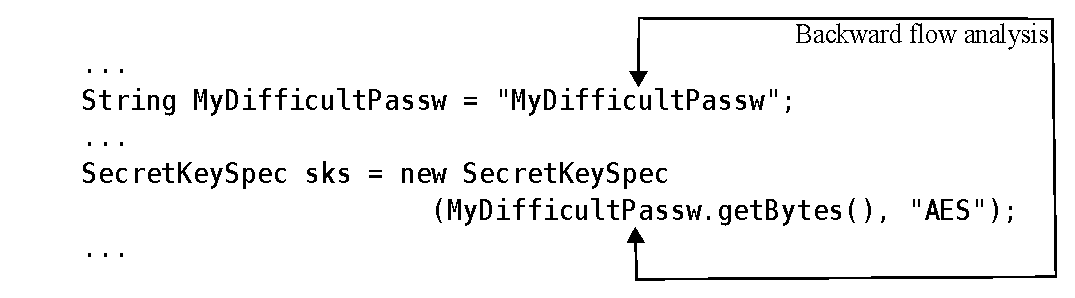
\includegraphics[width=\linewidth]{Figures/bckfwanalysis.eps}
\caption{An example showing how backward flow analysis can track 
the 1st parameter of \texttt{SecretKeySpec}, 
and identifies that it is statically defined by following back edges in the CFG}
\label{fig:slicing}
\end{figure}

%\minote{Here give one example explaining how you have choosen the slicing criteria, and the backward flow analysis. Then say example codes for other 
%rules are given in the appendix}
%The backward flow analysis starts a def-use analysis from the specified special function invokation place.    
% Talk why keyword based analysis can find FP. Also it would be better to show one code snippet in the start and refer it throughout the paper.
% Wrtie the lemma here that why FP will introduce no FP if the FP is with the the same procedure.
% Wait I could have used CryptoGuard to detect the inseucre patterns.. right?  

%\subsection{Synthesizing secure patterns}
\section{Results}
\section{Results}
\label{sec:results}
In this section, we will first describe our data-collection process. Next we will show the code repair, 
and detection accuracy techniques on a small subset of this collected dataset.   

\subsection{Data collection} 
  For experimental evaluation, We turn to the datasets from two previous sources ~\cite{meng2018secure,fischer2017stack}. 
  Both of these dataset contain code snippets posted on Stack Overflow. 
  Fisher et al. crawled 1,161 code snippets posted on Stack Overflow related to Andrioid security ~\cite{fischer2017stack}. 
  They considered a code snippet related to Android security if the code snippets makes API calls to
  one of the security services such as Java cryptography, Java secure communications, public key infrastructure X.509 certificates, 
  and Java authentication - authorization services. The popular crypto libraries used by Andriod developers such as Bouncy Castle, 
  SpongyCastle, Apache TLS/SSL, keyczar, jasypt, and GNU Crypto were also included. 
  
  Meng et al.  extracted 503 code snippets from 22,195 Stack Overflow posts by filtering the posts based on votes, duplications, 
  and absence of code snipeets~\cite{meng2018secure}. In total the dataset used in this experiments,  is generated by combining these two. 
  Our dataset contains 1,664 code snippets. The timeline of these code snippets are from 2008-2017.
  %\minote{add some more info and some statistics}
 % Since it would very time consuming to manually analysis 1.6K code snippets to get the ground truth, 
  %we randomly sample  half of the code snippets from the available corpus which is 800. 
  Upon manual inspection we filter out 363 as they were not related to security, and carry the experimental evaluation on 1273 code snippets 
  For the rest of the experiments we will only consider these 1301 code snippets.
    The average size of these %800 
  code snippets is 46 LoC having a very high standard deviation of 58. 


%\subsection{Data processing and categorization}
%  We manually analysis 
%  As to get the ground truth of the presence of insecure pattern, we have to manully analysis them, it becomes very time consuming. Therefore to make the analysis less consuming time , we only consider randomly sampled 800 code snippets -- about half of the 1.6K code snippets available. 
%  We then assign the code snippets into one of the 8 insecure patterns.  %and record the common keywords appear in the code snippets. By doing this we have list of common keyword for each of the 8 insecure patterns. We can then categorize all 1.6K code snippets using these common keywords.
  

\subsection{Code repair success rate.} 
%AES: 85/225 Broken-Hash: 69/219 
% Constructor class
\begin{figure}[ht]
  \includegraphics[width=\linewidth]{Figures/success_full_repair2.eps.eps}
  \caption{Percentage of code snippets successfully repaired. For each insecure pattern, we show the number 
  of code snippets we are able to convert to Jimple IR before and after applying code repairing.}
  \label{fig:code-repair}
\end{figure}

We call a code snippet successfully repaired if after applying the code repair techniques, we can convert it to a Jimple IR. 
We are able to convert 714 code snippets out of 1273 code snippets we have considered-- out which 401 of them was throwing exceptions
while converting them Jimple IR without any code repairs.  
Figure~\ref{fig:code-repair} 
illustrates the percentage of code snippets for each categorize, we have been able to parsed (i.e., convert to Jimple IR) before and after
the code repair techniques discussed in section~\ref{subsec:code-repair}.
In summary , we are able to parse 33\% more code snippets by code repairing.

%a repair accurarcy of 30.31\%. 
%We also categorize each converted into one more or category based on the secure/insecure use of the patterns presented on Table~\ref{tab:insecure-patterns}.  



\subsection{Insecure pattern detection accuracy.}
After converting each successfully repaired code snippets to Jimple IR, we detect insecure pattern 7, and 8 using keyword searching as mentioned previously. 
However for insecure pattern 1-6, need to apply backward flow analysis. To do this we give the Jimple IR to our tool. 
Out tool is built on top of CryptoGuard. 
CryptoGuard uses Soot as its program analysis engine. 
Using Soot's \texttt{JimpleAST} API~\footnote{\url{https://www.sable.mcgill.ca/soot/doc/soot/jimple/parser/JimpleAST.html}}, 
we can run backward flow analysis given the slicing criteria from Table~\ref{tab:slicing}. 
The idea is track the special method invocations parameter from the slicing criteria. 
In this way we can inspect the set of program statements which are affected 
by this slicing criteria, and figure out the presence of insecure patterns.



Table~\ref{tab:results} shows the total number of code snippets for of the 8 insecure patterns. 
%(they sum up to more than 813 as some code snippets has two or more rules). 
Parsed column refers to the number of code snippets, we have been able to convert to Jimple IR after applying the code repair discussed 
in section~\ref{subsec:code-repair}. We also shows the TP, FN, FN along side the precision, and recall rate.
As it can seen we have not been able to run backward flow analysis for insecure pattern 3. 
The reasons are explain the in the appendix~\ref{appendix:X509TrustManager}.
%If any of these set of program statements contains i) 
% Say you have done the  1,2,4,5, 7,8 correctely. How to present the results? 
% say you haven trying to address the problem of empty method detection but have not been able to do so. 

% Precision = tp/ (tp + fp)
% Recall = tp/ (tp + fn)

\begin{table}[ht]
\begin{tabular}{|c|r|r|r|r|r|r|r|}
\toprule
Insecure  Pattern \# & Parsed & TP & FP & FN & Precision & Recall \\ \midrule
1 & 225 & 186 & 39 & 0 & 100 & 82 \\
2 & 173 & 165 & 0 & 8 & 95 & 100 \\
\textcolor{red}{3} & \textcolor{red}{219} & \textcolor{red}{-} & \textcolor{red}{-} & \textcolor{red}{-} & \textcolor{red}{-} & \textcolor{red}{-}\\
4 & 68 & 61 &  0 & 8& 88 & 100 \\
5 & 40 & 37 & 0 & 3& 93 & 100 \\
6 & 90 & 81 & 7 & 2 & 91 & 91 \\ \midrule
7 & 68 & 63 & 0& 5 & 79 & 100 \\
8 & 20 & 11 & 0& 9 & 55 & 100\\ %\midrule 
%Total & 20 & 11 & 3& 0 & - & -\\        
\bottomrule
\end{tabular}
\caption{Precision and Recall of our analysis. Insecure pattern \#[7-8] where detected using keyword
searching. Insecure pattern \#[1-6] is detected using backward flow analysis. We are unable to detect
insecure pattern \#3 which is explained in appendix~\ref{appendix:X509TrustManager} 
}
\label{tab:results}
\end{table}


As we choose conservative keywords to  detect insecure pattern \#[7-8], 
both of them fails to detect cases some cases where insecure patterns occurs i.e., low precision. 
For backward flow analysis based detection inseucre patterns \#[1-6] has high accuracy and recall rate.      
\section{Limitations}
%\begin{itemize}
\item We did not analyze other code snippets other than Stack Overflow
\item Program repairs are basically simple parsing.
\item Limitations due to PPA/Jimple grammer. Could have used Eclispe JDT
\item The categoriezation is based on keyword searching.
\end{itemize}
\section{Discussions}
%
\section{Discussions on ML based detection techniques}
\label{sec:discussion}
%\subsection{ML based detection techniques.} 
Identification of insecure patterns, vulnerabilities, and code-smells using ML based 
techniques have been gaining tractions recently. This is mainly for two reasons 
i) leveraging the wealth of open source code available ii) adaptive neural network models 
which can capture/represent the complex patterns of source code. While givng a overview of ongoing  research in this area is outside
the scope of the paper, we can mention some work exciting research work closely related to ours that uses ML techniques. 
For example, Zhou et al. proposed~\cite{devign_neurips19} vulnerability detection model ``Devign'' for code snippets in C language. 
Their key idea to detect vulnerability is by capturing the abstract syntax tree structure of the source code via Gated-Graph Neural Network (GGNN).
The study in~\cite{Automated-Vulnerability-Detection-in-Source-Code-Using-Deep-Representation-Learning} proposed automated vulnerability detection 
tools using deep feature representation learning. 
%Interesting the study in~\cite{} hinted at detecting the issue of subjectivity the machine learning models suffers for detectin code smells by replicating the work in~\cite{}.

One problem associated with using machine learning models is that either they are function level detection 
model~\cite{Automated-Vulnerability-Detection-in-Source-Code-Using-Deep-Representation-Learning}, 
do have limited ability 
to reason why source code is vulnerable~\cite{devign_neurips19}, or suffers from subjectivity~\cite{are-we-there-yet}.


Static analysis based approaches such as ours, can overcome for two reasons i) it can reason about the source code, and ii) as insecure patterns are repetitive. As a result we can build a static analysis tool by observing 
the common insecure trends to reason about the  source. 
We agree this can be an overstretched claim, and leave it as a future work this paper.  
%\paragraph{Sythesis}


\iffalse
\subsection{ML based detection techniques}
\subsection{Code Repair}
\subsection{Limitations for failing to construct a CFG:} program repair are basically simple edits
PPA is very old

The tension between soundness and completeness: 
Our tool is the analysis part but not complete. but keyword based analysis also should introduce no FP. 
Synthesis
Other Sources of vulnerability: 
Lack of training /Knowledge: Vulnerable Online Turorials 
Lack of screening tools:
Being short and focusing on a working solution while writing code snippets.
\fi
\section{Related work}
%Finish the related work after gosol.
\section{Related Work}
\label{sec:related-work}
%\textbf{Code snippets on StackOverflow.} 
Our work is motived by the following related research work. 
Subramanian, et al.~\cite{subramanian2013making} used Eclipse Java Development Tools (JDT)~\footnote{\url{http://www.eclipse.org/jdt}}  
to find structural models of code snippets in Stack Overflow. Consequently, by analyzing \textit{solved} Stack Overflow questions having \textit{Android} tag they present a common list of Android API types and methods -- something which normal lexical parsers are unable to detect. 
Fischer et al.~\cite{fischer2017stack}  quantitatively evaluated the observation that a large number of insecure code snippets are being directly copy-pasted, repeatedly resued. They showed that a simple stochastic gradient descent based classifier can confirm that among 1.3 million Google Play Android applications, 15.4\% contains security-related code snippets from  from Stack Overflow -- out of which 97.9\% contain at least one insecre code snippet. 
Meng et al.~\cite{meng2018secure} did an empirical study on the on StackOverflow posts, aiming to understand developers’ concerns on Java secure coding. This study highlights a number of popular-accepted insecure suggestions on  StackOverflow including sugeestions to disabling the default protection against Cross-Site Request Forgery (CSRF) attacks, breaking SSL/TLS security through bypassing certificate validation, and using insecure cryptographic hash functions. These harmful insecure suggestions can easily misguide developer -- the extend of which is still unknown today. 
Interestingly, Rahman et al.~\cite{akondsnakes} did a study similar to Meng et al.~\cite{meng2018secure}, but for code snippets for Python language. They observed that 9.8\% of the 7,444 accepted answers to include at least one insecure code block. Most importantly they also find user reputation not
translate to the presence of insecure code blocks, implying  that both high and low-reputed users are likely to introduce insecure code blocks. 

%\noindent
%\textbf{Stackoverflow niye research}

%\noindent
%\textbf{Crypto abuse detection niye research}

\section{Future work and conclusions}
%
\section{Future work on Synthesizing secure code}
\label{sec:future-work}
// add something.
\bibliographystyle{ACM-Reference-Format}
\bibliography{references}
  
\section{Appendix}
\minote{This is working..}
\begin{lstlisting}[caption={A real code snippet taken from Stackoverflow. I want to build a tool which after analyzing the code snippet will highlight the part of the code that is insecure and suggest an alternative secure implementation as showed in the figure.}, label={fig:motivating-example}]
    private byte[] encrypt(byte[] raw, byte[] clear) {
      ...
      _Cipher cipher = Cipher.getInstance("AES")_;}
      // Cipher cipher = Cipher.getInstance("AES/CBC/PKCS5Padding");
      ....
      return encrypted
    }
     \end{lstlisting}
% evalutation plan on datasets.
\end{document}
\end{document}